\section{Cơ sở lý thuyết}
\subsection{Tổng quan về Ngành Du lịch và Lữ hành}
\subsubsection{Cấu trúc Ngành Du lịch và Lữ hành}
Theo định nghĩa về Lữ hành tại khoản 1 Điều 3 của Luật Du lịch 2017, Lữ hành là thuật ngữ chỉ các hoạt động du lịch liên quan đến những chuyến đi của con người ngoài nơi cư trú thường xuyên trong khoảng thời gian không quá 1 năm liên tục. Du lịch là hoạt động đi ra khỏi nơi cư trú thường xuyên trong thời gian không quá một năm nhằm mục đích nghỉ dưỡng, giải trí, tham quan, khám phá tài nguyên du lịch hoặc kết hợp mục đích hợp pháp khác

Ngành du lịch được cấu thành từ nhiều lĩnh vực liên kết chặt chẽ:
\begin{itemize}
    \item \textbf{Vận chuyển (Transportation)}: Bao gồm hàng không, đường sắt, đường bộ (xe buýt, ô tô cá nhân, xe cho thuê), và đường thủy (tàu du lịch, phà). Đây là yếu tố nền tảng cho sự di chuyển của du khách.
    \item \textbf{Lưu trú (Accommodation)}: Gồm khách sạn, khu nghỉ dưỡng (resorts), nhà nghỉ, căn hộ dịch vụ, homestay, và các nền tảng chia sẻ như Airbnb. Đây là nơi du khách ở lại trong suốt chuyến đi.
    \item \textbf{Điểm tham quan và Hoạt động (Attractions \& Activities)}: Bao gồm các tài nguyên thiên nhiên (bãi biển, công viên quốc gia), di sản văn hóa (bảo tàng, di tích lịch sử), công trình nhân tạo (công viên giải trí, trung tâm mua sắm), và các hoạt động trải nghiệm (lớp học nấu ăn, tour đi bộ, thể thao mạo hiểm).
    \item \textbf{Dịch vụ Ăn uống (Food \& Beverage)}: Nhà hàng, quán cà phê, quán bar, dịch vụ ăn uống tại nơi lưu trú.
    \item \textbf{Dịch vụ Lữ hành (Travel Services)}: Các đơn vị trung gian kết nối du khách với các nhà cung cấp dịch vụ, bao gồm đại lý du lịch, công ty tổ chức tour, và các nền tảng trực tuyến.
\end{itemize}

\subsubsection{Các mô hình kinh doanh chủ đạo}
\begin{enumerate}
    \item Đại lý Du lịch (Travel Agency):
        \begin{itemize}
            \item Truyền thống (Traditional): Các văn phòng, tư vấn trực tiếp cho khách hàng, đóng vai trò trung gian bán lẻ sản phẩm của các nhà cung cấp (vé máy bay, phòng khách sạn, tour).
            \item Trực tuyến (Online Travel Agency - OTA): Các nền tảng kỹ thuật số (ví dụ: Booking.com, Agoda, Expedia) cho phép khách hàng tự tìm kiếm, so sánh và đặt dịch vụ. OTA có quy mô toàn cầu, dữ liệu lớn và khả năng tiếp cận khách hàng rộng khắp.
        \end{itemize}
    \item Công ty Tổ chức Tour (Tour Operator): Các công ty này chủ động xây dựng, đóng gói các sản phẩm du lịch trọn gói (package tours) bao gồm vận chuyển, lưu trú, ăn uống, hướng dẫn viên và lịch trình tham quan. Họ bán sản phẩm này trực tiếp hoặc thông qua các đại lý du lịch.
    \item Dịch vụ Du lịch Cá nhân hóa và Nền tảng Chia sẻ:
        \begin{itemize}
            \item Cá nhân hóa (Personalized Travel Services): Các dịch vụ thiết kế hành trình theo yêu cầu riêng của từng khách hàng, tập trung vào trải nghiệm độc đáo và chuyên sâu.
            \item Nền tảng Kinh tế Chia sẻ (Sharing Economy Platforms): Các nền tảng như Airbnb (lưu trú), GetYourGuide (hoạt động tại điểm đến) cho phép các cá nhân hoặc doanh nghiệp nhỏ cung cấp dịch vụ trực tiếp đến du khách, tạo ra sự đa dạng và cạnh tranh.
        \end{itemize}
\end{enumerate}

\subsubsection{Khách hàng mục tiêu và Phân khúc}
Sự khác biệt trong nhu cầu lập kế hoạch của từng phân khúc là cơ sở quan trọng để cá nhân hóa gợi ý.
\begin{itemize}
    \item Du lịch Tự túc/Bụi (Backpacking/Independent Travel): Khách hàng quan tâm về ngân sách, linh hoạt về thời gian, ưu tiên trải nghiệm địa phương và tính xác thực. Họ cần thông tin chi tiết, các mẹo tiết kiệm chi phí, và các gợi ý về những điểm đến "hidden" ít người biết.
    \item Du lịch Nghỉ dưỡng (Leisure/Resort Travel): Khách hàng tìm kiếm sự thư giãn, tiện nghi và dịch vụ trọn gói. Họ quan tâm đến chất lượng của nơi lưu trú, các hoạt động giải trí tại chỗ và sự thuận tiện trong việc đi lại.
    \item Du lịch Công vụ (Business Travel): Khách hàng có lịch trình chặt chẽ, ưu tiên hiệu quả, sự thuận tiện về địa điểm (gần nơi họp, sân bay), và các dịch vụ hỗ trợ công việc (Wi-Fi, phòng họp).
    \item Du lịch Gia đình (Family Travel): Khách hàng ưu tiên các điểm đến và hoạt động an toàn, phù hợp với trẻ em, các lựa chọn lưu trú và ăn uống thân thiện với gia đình.
\end{itemize}

\subsubsection{Chuỗi cung ứng Dịch vụ Du lịch}
Chuỗi cung ứng du lịch (Tourism Supply Chain - TSC) là một mạng lưới các tổ chức du lịch tham gia vào các hoạt động khác nhau (như vận tải, lưu trú, ăn uống, mua sắm, giải trí), từ cung cấp các thành phần khác nhau của các sản phẩm hoặc dịch vụ du lịch như các chuyến bay và chỗ ở cho đến việc phân phối và tiếp thị sản phẩm du lịch cuối cùng tại một điểm đến cụ thể, và có sự tham gia của nhiều cá nhân hoặc tổ chức trong cả lĩnh vực tư nhân và công cộng [].

Các thành phần trong chuỗi cung ứng gồm:
\begin{itemize}
    \item Nhà Cung cấp (Suppliers): Các đơn vị sở hữu và vận hành dịch vụ cốt lõi (hãng hàng không, khách sạn, công ty vận tải, ban quản lý điểm tham quan).
    \item Đơn vị trung gian (Intermediaries): Nhà tổ chức tour - Kết hợp các dịch vụ riêng lẻ thành một gói hoàn chỉnh. Đại lý du lịch/OTA - Phân phối và bán lẻ các dịch vụ hoặc gói tour đến khách hàng. Họ đóng vai trò quan trọng trong việc tổng hợp thông tin và cung cấp công cụ tìm kiếm, so sánh.
    \item Khách hàng (Customers): Người sử dụng cuối cùng của dịch vụ. Họ là nguồn cung cấp dữ liệu quan trọng (sở thích, hành vi, đánh giá) để cải thiện chuỗi cung ứng.
\end{itemize}

\subsection{Hành trình Khách hàng (Customer Journey) trong Du lịch}
\subsubsection{Định nghĩa}
Hành trình khách hàng trong du lịch là toàn bộ quá trình mà một người trải qua từ khi nảy sinh ý định đi du lịch cho đến khi kết thúc chuyến đi và chia sẻ kỷ niệm. Quá trình này thường được chia thành 5 giai đoạn chính:
\begin{enumerate}
    \item Giai đoạn Ước mơ (Dreaming/Inspiration): Khách hàng bắt đầu hình thành ý tưởng về một chuyến đi, thường được truyền cảm hứng từ mạng xã hội, bạn bè, phim ảnh, hoặc các bài viết du lịch. Nhu cầu thông tin ở giai đoạn này là những hình ảnh, câu chuyện hấp dẫn, mang tính gợi mở.
    \item Giai đoạn Lập kế hoạch (Planning): Khách hàng đã quyết định được điểm điến và bắt đầu sắp xếp một lịch trình cụ thể: chọn ngày đi, quyết định thứ tự tham quan các địa điểm, ước tính thời gian và ngân sách. Khách hàng tích cực tìm kiếm thông tin về địa điểm, so sánh chi phí, đọc đánh giá, xem các lựa chọn về vận chuyển và lưu trú.
    \item Giai đoạn Đặt dịch vụ (Booking): Khách hàng tiến hành thanh toán cho các dịch vụ đã chọn như vé máy bay, phòng khách sạn, tour trong ngày. Nhu cầu là một quy trình đặt dịch vụ đơn giản, an toàn và minh bạch.
    \item Giai đoạn Trải nghiệm (Experiencing): Khách hàng thực sự tham gia vào chuyến đi. Nhu cầu của họ là các thông tin theo thời gian thực như chỉ đường, gợi ý quán ăn gần đây, thông tin về thời tiết, hoặc điều chỉnh lịch trình đột xuất.
    \item Giai đoạn Chia sẻ (Sharing): Sau chuyến đi, khách hàng chia sẻ trải nghiệm, hình ảnh, video và viết đánh giá trên các nền tảng mạng xã hội hoặc website du lịch. Nội dung này trở thành nguồn cảm hứng và thông tin cho những người khác.
\end{enumerate}

\begin{figure}[h!]
    \centering
    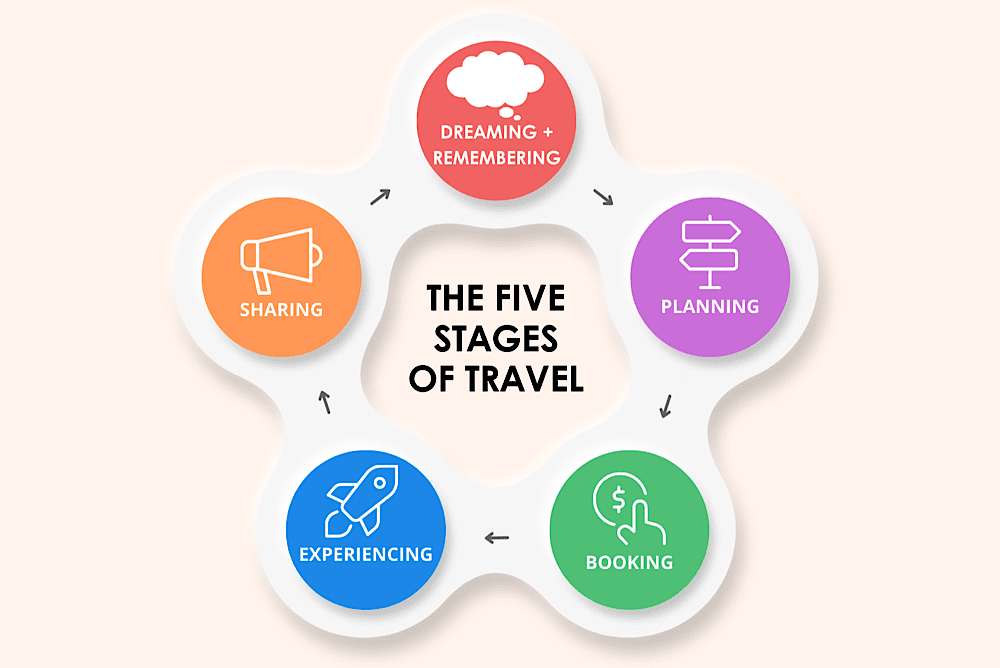
\includegraphics[width=13 cm]{Images/2-knowledge/customer-journey.png}
    \caption{5 Giai đoạn của Hành trình khách hàng trong du lịch}
    \label{fig:placeholder}
\end{figure}

\subsubsection{Vai trò của Gợi ý Hành trình dựa trên AI}
Hệ thống gợi ý hành trình dựa trên AI có thể can thiệp hiệu quả vào nhiều giai đoạn, nhưng đặc biệt quan trọng ở giai đoạn Lập kế hoạch (Planning) sau:
\begin{itemize}
    \item Điểm chạm (Touchpoint): Công cụ tìm kiếm, blog du lịch, trang web của OTA, bảng tính, sổ tay, các công cụ lập kế hoạch trực tuyến.
    \item Khó khăn (Pain Point): Quá tải thông tin, thông tin bị phân mảnh, khó xác minh độ tin cậy của nguồn tin, mất thời gian để tổng hợp và so sánh. Khó khăn trong việc tối ưu hóa lịch trình (thứ tự địa điểm, thời gian di chuyển), không biết cách sắp xếp các hoạt động một cách logic, bỏ lỡ những điểm đến thú vị.
    \item Giải pháp của AI: Hệ thống có thể cung cấp các gợi ý điểm đến được cá nhân hóa dựa trên hồ sơ người dùng (sở thích, ngân sách, lịch sử du lịch), giúp thu hẹp phạm vi tìm kiếm và đưa ra những lựa chọn phù hợp ngay từ đầu. Tự động tạo ra một hoặc nhiều phương án lịch trình hoàn chỉnh dựa trên các tiêu chí đầu vào (số ngày, danh sách địa điểm mong muốn, phong cách du lịch). Áp dụng các thuật toán để giải quyết các bài toán như "Người bán hàng du lịch" (TSP) nhằm tìm ra lộ trình di chuyển hiệu quả nhất về thời gian và chi phí. Gợi ý các hoạt động, nhà hàng dựa trên phân tích dữ liệu từ đánh giá của những người dùng có cùng sở thích.
\end{itemize}

\subsection{Cơ sở Kỹ thuật và Công nghệ}
\subsubsection{Hệ thống Gợi ý}
Hệ thống gợi ý là một lớp con của hệ thống lọc thông tin, có nhiệm vụ dự đoán "sự yêu thích" hoặc "sở thích" mà một người dùng có thể dành cho một mục (item), và từ đó đề xuất những mục phù hợp nhất.

Phân loại chính và ứng dụng trong gợi ý hành trình:
\begin{itemize}
    \item Lọc dựa trên Nội dung (Content-Based Filtering): Gợi ý các mục tương tự như những mục người dùng đã thích trong quá khứ. Ví dụ trong du lịch: Nếu người dùng thích "Bảo tàng Lịch sử" và "Di tích Nhà tù Côn Đảo", hệ thống sẽ gợi ý các địa điểm có thuộc tính tương tự như "di tích lịch sử", "văn hóa".
    \item Lọc Cộng tác (Collaborative Filtering): Gợi ý dựa trên sở thích của những người dùng tương tự.
        \begin{itemize}
            \item User-based CF: Tìm những người dùng có cùng "khẩu vị" (ví dụ: cùng thích du lịch mạo hiểm, cùng đánh giá cao các homestay) và gợi ý những địa điểm mà người dùng tương tự đã thích.
            \item Item-based CF: Tìm sự tương quan giữa các địa điểm. Ví dụ, những người đã đến "Mũi Nghinh Phong" cũng thường đến "Tượng Chúa Kitô Vua", từ đó gợi ý cho người dùng đang quan tâm đến một trong hai địa điểm.
        \end{itemize}
    \item Hệ thống Lai (Hybrid Systems): Kết hợp hai hoặc nhiều phương pháp trên để khắc phục nhược điểm của từng phương pháp (như vấn đề "khởi đầu lạnh" - cold start) và tăng độ chính xác. Đây là hướng tiếp cận phổ biến và hiệu quả nhất cho các hệ thống phức tạp như gợi ý hành trình.
\end{itemize}

\subsubsection{Trí tuệ Nhân tạo (AI) và Machine Learning (ML)}
AI/ML là công nghệ lõi cho phép hệ thống "học" từ dữ liệu để đưa ra các quyết định thông minh.
\begin{itemize}
    \item Phân tích Dữ liệu Du lịch: Xử lý và phân tích khối lượng lớn dữ liệu phi cấu trúc (đánh giá, hình ảnh) và có cấu trúc (thông tin địa điểm, dữ liệu đặt chỗ) để tìm ra các mẫu hành vi và sở thích ẩn.
    \item Cá nhân hóa Gợi ý: Xây dựng mô hình hồ sơ người dùng (user profile) động, cập nhật liên tục dựa trên tương tác của họ với hệ thống, từ đó điều chỉnh các gợi ý cho phù hợp.
    \item Xây dựng Thuật toán Tối ưu hóa: Giải quyết các bài toán tối ưu hóa tổ hợp phức tạp. Ví dụ kinh điển là Bài toán Người bán hàng du lịch (Traveling Salesman Problem - TSP): cho một danh sách các thành phố (điểm tham quan) và khoảng cách giữa chúng, tìm chu trình ngắn nhất đi qua mỗi thành phố đúng một lần và quay về điểm xuất phát. Trong gợi ý hành trình, TSP được dùng để tối ưu hóa lộ trình di chuyển giữa các điểm đến trong một ngày, giúp tiết kiệm thời gian và chi phí.
\end{itemize}

\subsubsection{Các Thuật ngữ Kỹ thuật Cốt lõi}
Hành trình Du lịch Tối ưu (Optimal Itinerary/Path): Là một lịch trình di chuyển và tham quan được xây dựng để tối đa hóa hoặc tối thiểu hóa một hoặc nhiều hàm mục tiêu. Các tiêu chí đánh giá sự tối ưu bao gồm:
\begin{itemize}
    \item Thời gian: Tổng thời gian di chuyển và tham quan ngắn nhất.
    \item Chi phí: Tổng chi phí di chuyển, vé vào cửa, và các chi phí liên quan là thấp nhất.
    \item Sự hài lòng (Satisfaction): Mức độ phù hợp của các điểm đến trong hành trình với sở thích của người dùng, dựa trên điểm đánh giá của cộng đồng và độ phổ biến.
\end{itemize}

Chất lượng Gợi ý (Recommendation Quality): Được đo lường bằng các chỉ số sau:
\begin{itemize}
    \item Độ chính xác (Precision): Tỷ lệ các mục được gợi ý mà người dùng thực sự quan tâm (TP: True Positive, FP: False Positive).
    \item Độ phủ (Recall/Sensitivity): Tỷ lệ các mục mà người dùng quan tâm được hệ thống gợi ý thành công (FN: False Negative).
    \item Độ bao phủ (Coverage): Khả năng của hệ thống gợi ý được nhiều loại mục khác nhau, tránh việc chỉ gợi ý các mục phổ biến.
    \item Tính mới lạ (Novelty): Khả năng gợi ý những mục mới, ít được biết đến nhưng có thể người dùng sẽ thích, giúp họ khám phá.
\end{itemize}

Trợ lý Du lịch Ảo (AI Travel Assistant): Là một ứng dụng hoặc tính năng tích hợp AI, thường dưới dạng chatbot hoặc giao diện hội thoại, có khả năng tương tác với người dùng bằng ngôn ngữ tự nhiên. Chức năng của nó bao gồm:
\begin{itemize}
    \item Thu thập yêu cầu và sở thích của người dùng.
    \item Trả lời các câu hỏi liên quan đến du lịch.
    \item Đề xuất và tùy chỉnh hành trình theo thời gian thực.
    \item Hỗ trợ đặt dịch vụ và cung cấp thông tin trợ giúp trong chuyến đi.
\end{itemize}

\subsection{Cơ sở về Đánh giá và Cộng đồng Người dùng}
Dữ liệu từ cộng đồng là thông tin quan trọng để hệ thống AI học và đưa ra các gợi ý thông minh, đáng tin cậy.

\subsubsection{Cộng đồng Du lịch Trực tuyến và UGC (User-Generated Content)}
UGC là bất kỳ dạng nội dung nào (văn bản, hình ảnh, video, đánh giá, bình luận) được tạo ra và chia sẻ bởi người dùng trên các nền tảng trực tuyến (TripAdvisor, Instagram, Facebook, các blog du lịch). UGC được coi là đáng tin cậy hơn so với nội dung quảng cáo từ nhà cung cấp dịch vụ vì nó phản ánh trải nghiệm thực tế. Các nội dung đánh giá và xếp hạng từ những người đi trước có tác động rất lớn đến quyết định lựa chọn điểm đến, khách sạn, nhà hàng của du khách. Đây là nguồn cung cấp dữ liệu chi tiết về các khía cạnh khác nhau của một dịch vụ, giúp hệ thống hiểu sâu hơn về chất lượng và đặc tính của từng địa điểm.

\subsubsection{Xử lý và Khai thác Dữ liệu Cộng đồng}
Để biến UGC từ dạng phi cấu trúc thành thông tin hữu ích cho hệ thống gợi ý, cần áp dụng các kỹ thuật Xử lý Ngôn ngữ Tự nhiên (NLP).
\begin{enumerate}
    \item Phân tích Cảm xúc (Sentiment Analysis): Là quá trình xác định và phân loại quan điểm, cảm xúc (tích cực, tiêu cực, trung tính) được thể hiện trong một đoạn văn bản. Ứng dụng: Tự động tính điểm cảm xúc cho mỗi đánh giá về một địa điểm. Thay vì chỉ dựa vào xếp hạng sao (ví dụ: 4/5 sao), hệ thống có thể hiểu được sắc thái trong bình luận, giúp xếp hạng địa điểm một cách chính xác hơn.
    \item Khai phá Ý kiến (Opinion Mining / Aspect-Based Sentiment Analysis): Là một dạng phân tích sâu hơn, không chỉ xác định cảm xúc chung mà còn xác định cảm xúc đó hướng về khía cạnh (aspect) cụ thể nào của sản phẩm/dịch vụ. 
    \begin{itemize}
        \item Với bình luận "Khách sạn này có hồ bơi rất đẹp nhưng bữa sáng thì tệ", hệ thống có thể trích xuất: /{aspect: "hồ bơi", sentiment: "tích cực"/}, /{aspect: "bữa sáng", sentiment: "tiêu cực"/}
        \item Ứng dụng: Thông tin này cực kỳ giá trị cho việc cá nhân hóa. Hệ thống có thể gợi ý một khách sạn cho người dùng ưu tiên "hồ bơi đẹp" và tránh gợi ý nó cho người dùng quan tâm đến "chất lượng bữa sáng". Điều này giúp tạo ra những gợi ý tinh vi và phù hợp hơn nhiều.
    \end{itemize}
\end{enumerate}




% []https://vietnambiz.vn/chuoi-cung-ung-du-lich-tourism-supply-chain-la-gi-20191210104810307.htm
